% tk-04 演示：√(x²+1) + √((x-3)²+4) 的最小值——数→形 + 将军饮马
% A(0,1), B(3,2)，P 在 x 轴上动；A' = (0,-1) 是 A 关于 x 轴对称点
\documentclass[tikz,border=4pt]{standalone}
\usepackage{ctex}
\usepackage{amsmath}
\usetikzlibrary{calc, arrows.meta}
\begin{document}
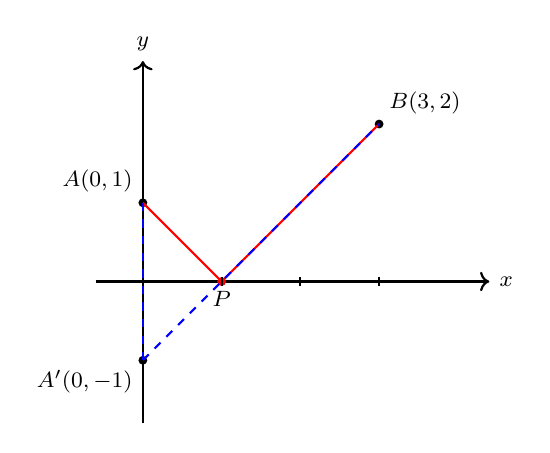
\begin{tikzpicture}[scale=1.0, thick]
  \draw[->] (-0.6,0) -- (4.4,0) node[right] {\footnotesize $x$};
  \draw[->] (0,-1.8) -- (0,2.8) node[above] {\footnotesize $y$};

  \coordinate (A)  at (0,1);
  \coordinate (Ap) at (0,-1);
  \coordinate (B)  at (3,2);
  % A'B 与 x 轴交点 P：参数化求 y=0 时 x
  % A'=(0,-1), B=(3,2), 方向 (3,3)；y=0: t = 1/3 -> x = 1
  \coordinate (P)  at (1,0);

  \fill (A)  circle (1.6pt);
  \fill (B)  circle (1.6pt);
  \fill (Ap) circle (1.6pt);
  \fill[red] (P) circle (1.6pt);

  % 距离
  \draw[red] (A) -- (P);
  \draw[red] (P) -- (B);
  % 对称：A 与 A'
  \draw[blue, dashed] (A) -- (Ap);
  % A'B 整段（说明 PA' + PB = A'B 最小）
  \draw[blue, dashed] (Ap) -- (B);

  \node[above left]  at (A)  {\footnotesize $A(0,1)$};
  \node[below left]  at (Ap) {\footnotesize $A'(0,-1)$};
  \node[above right] at (B)  {\footnotesize $B(3,2)$};
  \node[below]       at (P)  {\footnotesize $P$};

  % 刻度小标
  \foreach \x in {1,2,3} {
    \draw (\x,0.06) -- (\x,-0.06);
  }
\end{tikzpicture}
\end{document}
